\documentclass{article}
\usepackage{graphicx}
\usepackage{float}
\usepackage{subcaption}
\usepackage[font=small,labelfont=bf]{caption}
\usepackage[round,authoryear]{natbib}


\setlength{\textfloatsep}{8pt plus 2pt minus 2pt}
\setlength{\floatsep}{8pt plus 2pt minus 2pt}
\setlength{\intextsep}{8pt plus 2pt minus 2pt}

\title{BioClinical ModernBERT}
\author{Ikenna Ojoboh}


\begin{document}

\maketitle

\section{Methods}

We modelled PubMedQA as a single biomedical question answering pipeline that maps a question and its supporting abstract to one of three labels: \textit{yes}, \textit{no}, or \textit{maybe}. Our design followed a structured scientific-method and design-of-experiments approach: fix preprocessing and backbone first, optimise a strong supervised baseline, test one major improvement at a time, and retain only changes that improved downstream QA (Question Answering). Figure~\ref{fig:stage1_biomedicalbert} shows the Stage~1 route-selection logic, where masked adaptation training was tested but rejected in favour of the base model. The stronger base route was then fine-tuned on the PQA-A artificial weak-label dataset; Figure~\ref{fig:stage2_biomedicalbert} shows the final standardised Stage~2 evaluation protocol.

\begin{figure}[H]
    \centering
    \begin{subfigure}[t]{0.48\linewidth}
        \centering
        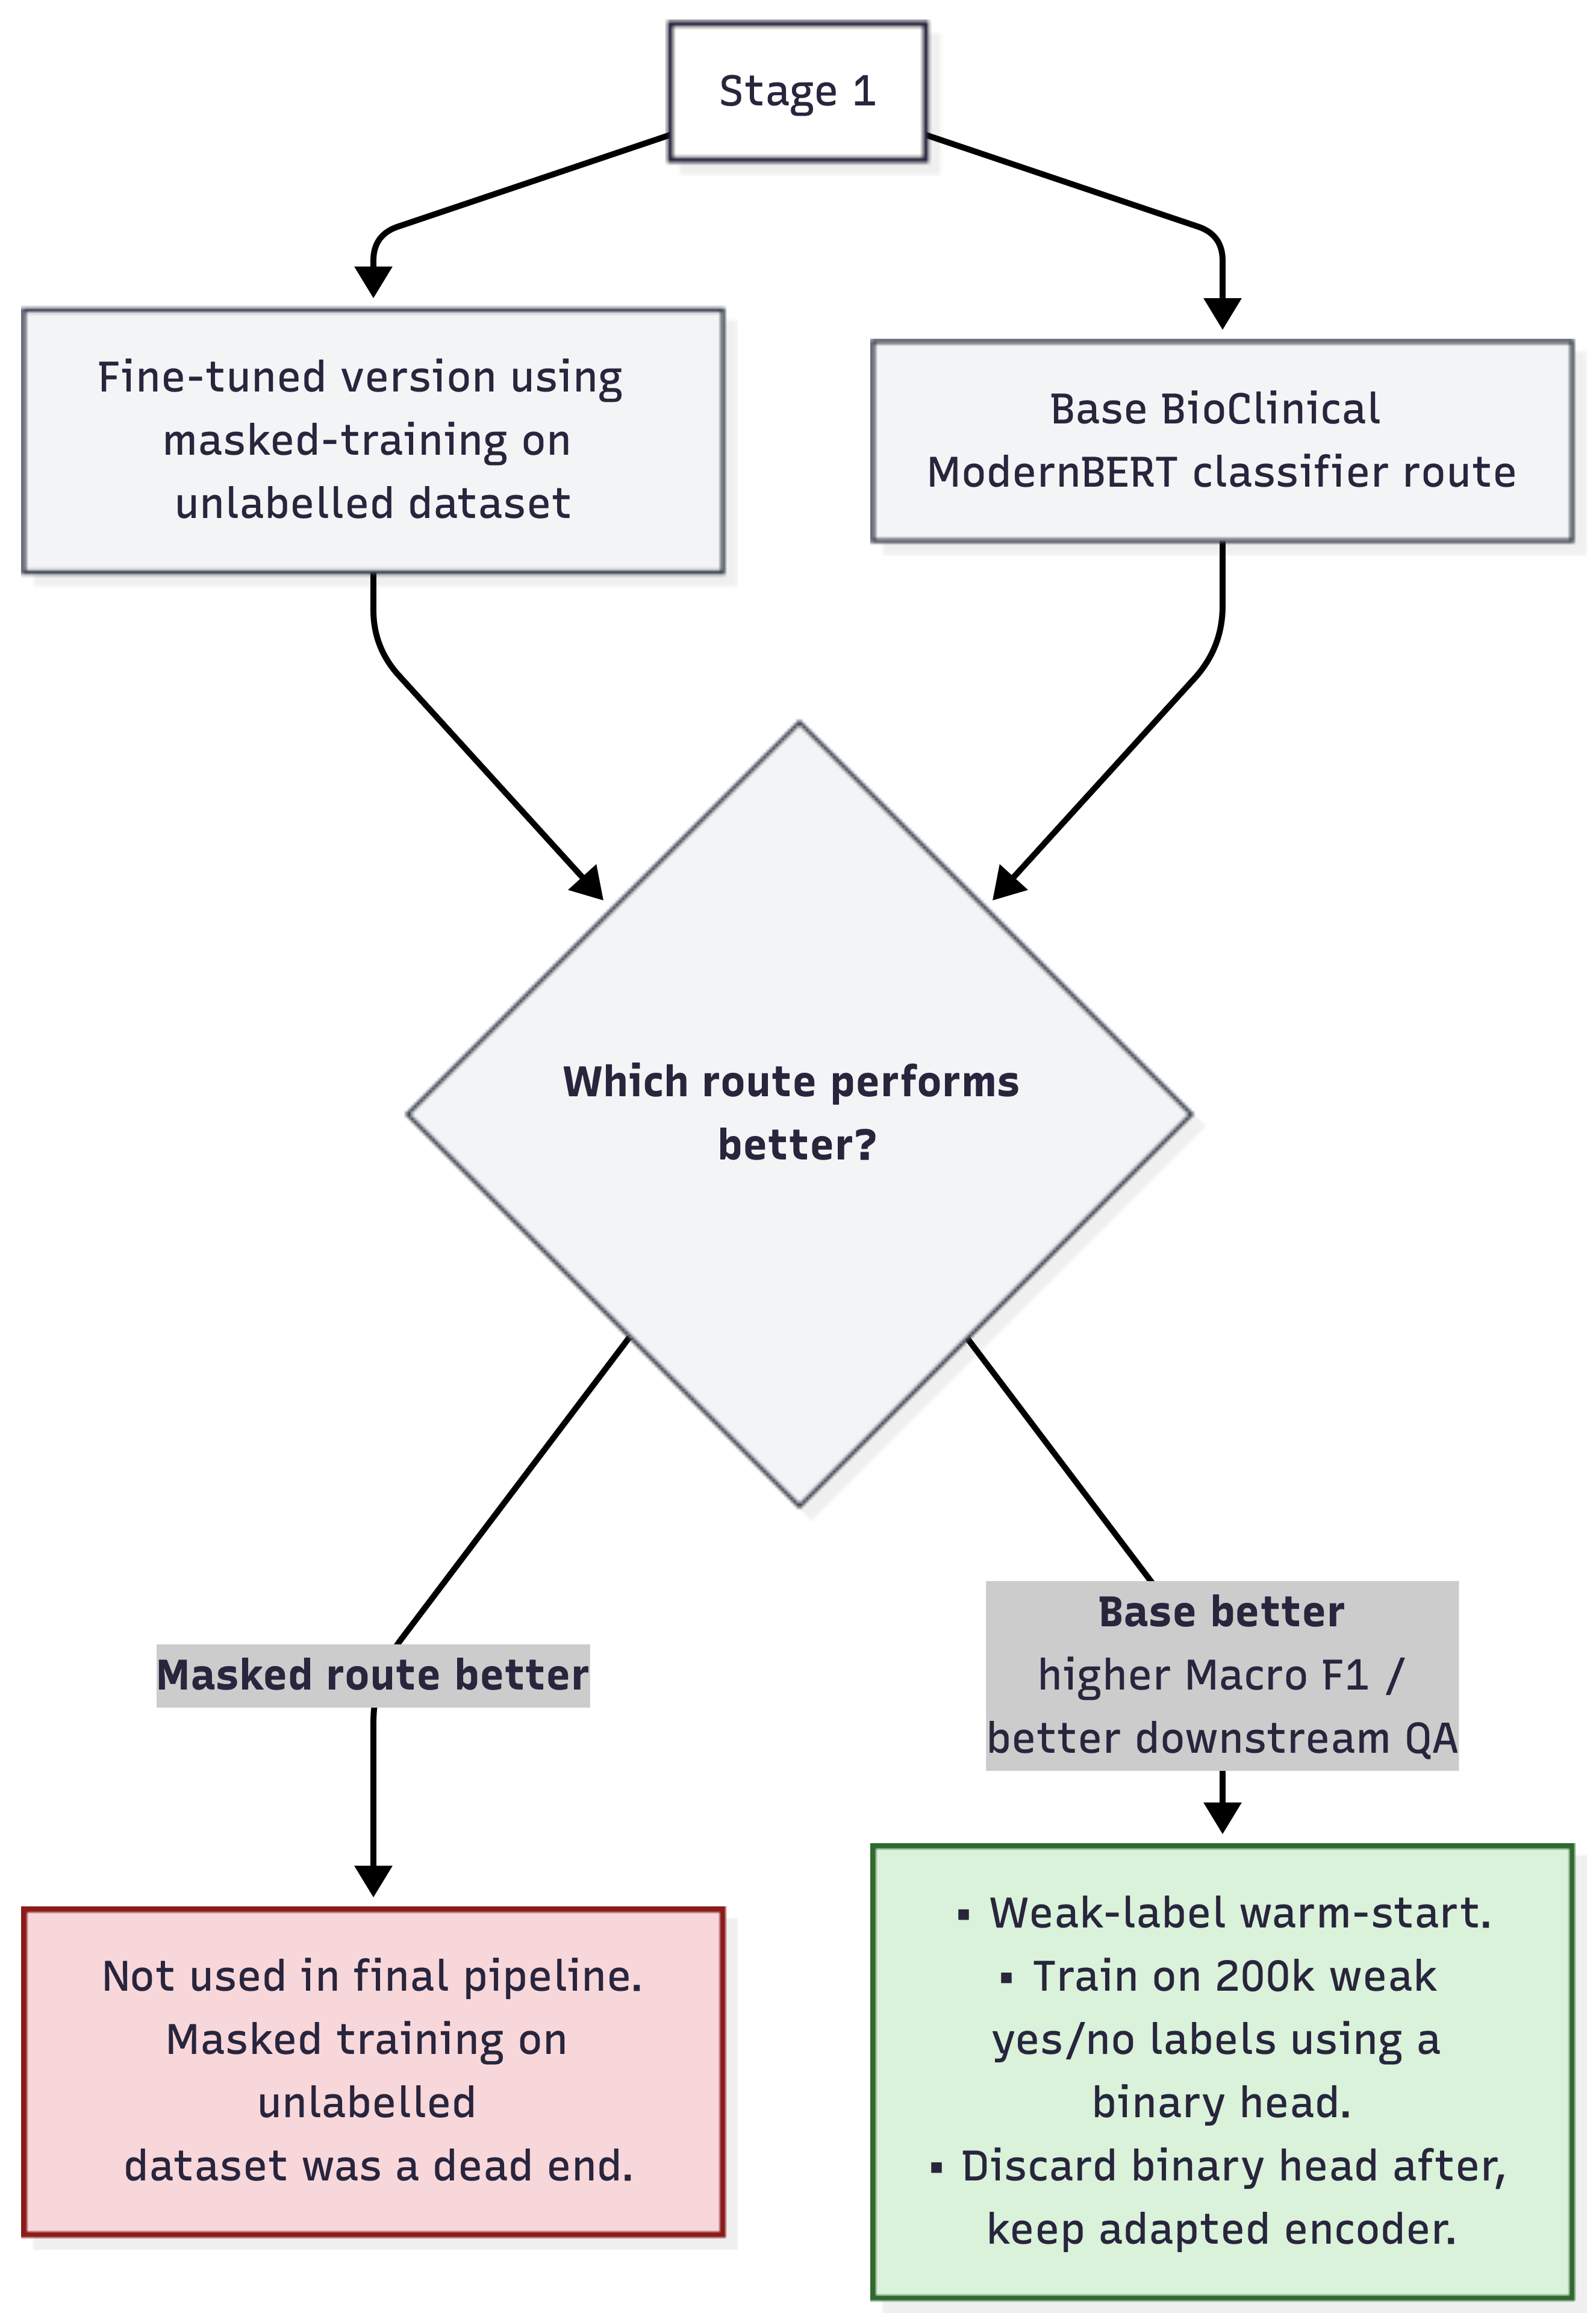
\includegraphics[width=\linewidth,height=0.78\textheight,keepaspectratio]{Stage1_AI.png}
        \caption{Stage~1 route selection and weak warm-start (PQA-A finetuning).}
        \label{fig:stage1_biomedicalbert}
    \end{subfigure}
    \hfill
    \begin{subfigure}[t]{0.48\linewidth}
        \centering
        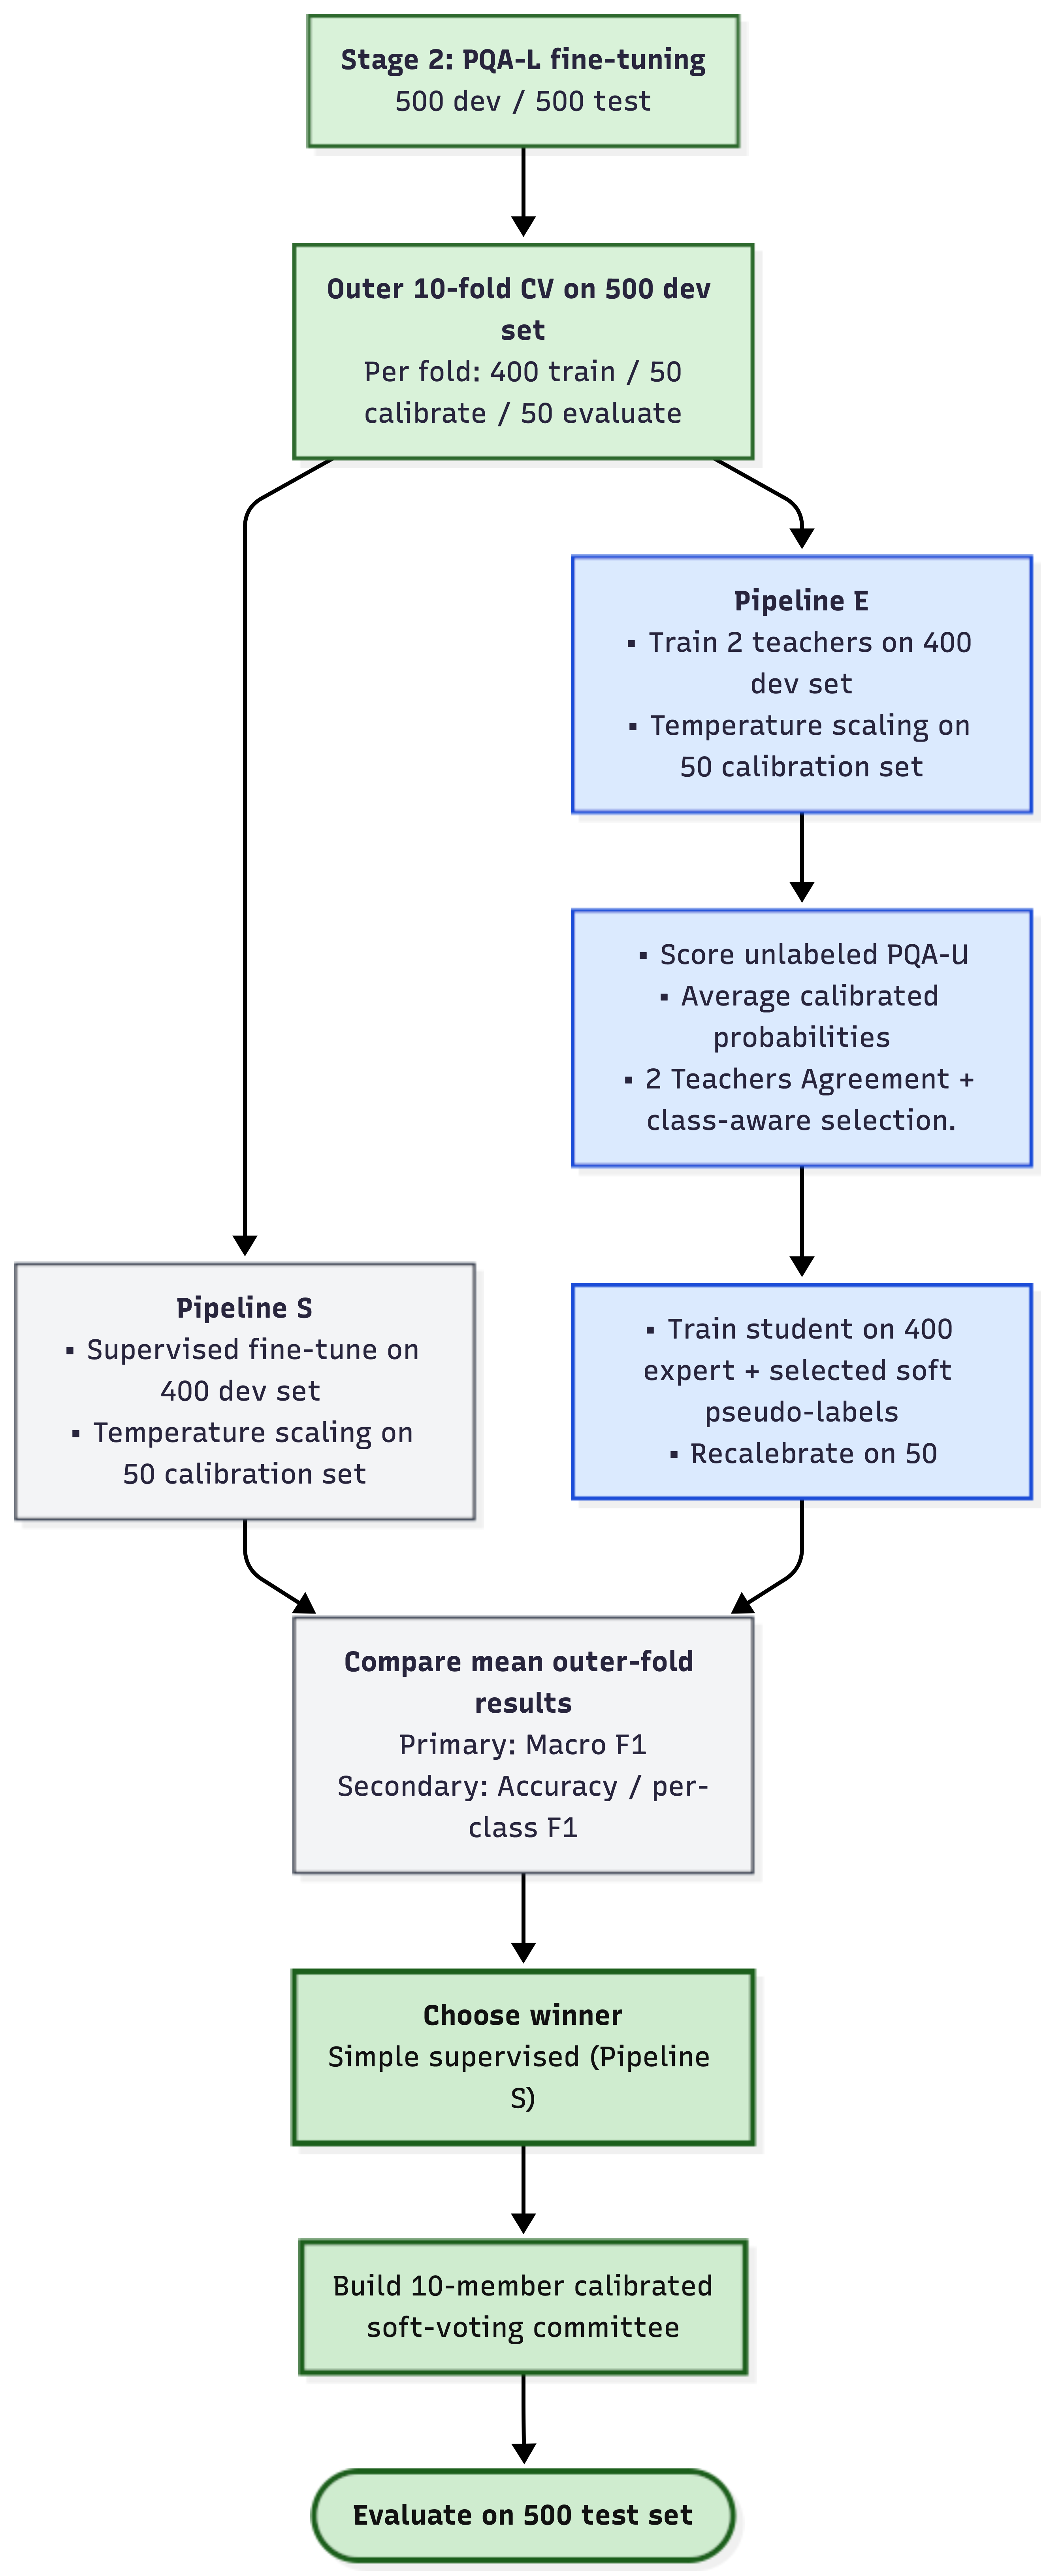
\includegraphics[width=\linewidth,height=0.78\textheight,keepaspectratio]{Stage2_AI.png}
        \caption{Stage~2 standardised 500/500 evaluation protocol.}
        \label{fig:stage2_biomedicalbert}
    \end{subfigure}
    \caption{BioClinical ModernBERT training and evaluation design.}
    \label{fig:biomedicalbert_overview}
\end{figure}

Each example was encoded as paired \texttt{QUESTION} and \texttt{CONTEXTS}, with all context strings concatenated into one text field. Labels were mapped as \texttt{no}=0, \texttt{maybe}=1, and \texttt{yes}=2. Tokenisation used paired encoding with truncation on the context side only so that the question was always preserved. We set \texttt{max\_length}=512 after analysing 5{,}000 expert-labelled examples: mean length was 302.08 tokens, median 300, the 95th percentile was 443.05, the 99th percentile was 538.02, and only 90/5000 examples (1.80\%) exceeded 512. This gave near-complete coverage without unnecessary memory cost. The final representation/model pair used \textbf{BioClinical ModernBERT} with a sequence-classification head, motivated by the expectation that a domain-specific biomedical transformer would capture long-range biomedical context and answer uncertainty better than shallower alternatives \citep{Gu2020,Warner2025}.

We first optimised a supervised BioClinical ModernBERT classifier. Early untuned runs showed strong majority-class bias, especially collapse on \textit{maybe}, so class imbalance became the main optimisation target. We compared plain fine-tuning, class-weighted loss, class-weighted loss plus weighted sampling, and weighted sampling alone, selecting models by validation macro F1 because raw accuracy masked minority-class failure \citep{Younes2022}. The best recipe used weighted sampling only, no class-weighted loss, learning rate $8\times10^{-6}$, gradient accumulation of 2, dynamic padding, early stopping, and checkpoint selection by validation macro F1. We also tested masked language model fine-tuning on the ulabelled PQA-U biomedical text as a possible improvement \citep{Gururangan2020}, but although MLM loss improved, downstream PubMedQA performance did not, and the route was far more memory-intensive on the available M1 Max / 32\,GB / MPS hardware. As shown in Figure~\ref{fig:stage1_biomedicalbert}, this branch was therefore rejected.

The surviving Stage~1 branch used a weak-to-strong design: the encoder was warm-started on approximately 200k weakly labelled binary \textit{yes/no} examples, after which the binary head was discarded and only the adapted encoder was retained. A pilot on a 10\% subset of the weak data was used to choose the Stage~1 recipe, which selected weighted sampling without class-weighted loss and a learning rate of $1\times10^{-5}$. This configuration was then used on the full PQA-A weak training, and the best checkpoint provided the warm-start encoder for Stage~2. Stage~2 then followed the standardised protocol in Figure~\ref{fig:stage2_biomedicalbert}. The 1,000 expert-labelled examples were split into 500 development and 500 test examples with matched class balance, and outer 10-fold cross-validation was run on the development half. Within each fold, data was divided into \textbf{400 train / 50 calibration / 50 evaluation}, which separated model fitting, probability calibration, and final fold evaluation.

Table~\ref{tab:bcb_main_protocol} summarises the two Stage~2 pipelines. \textbf{Pipeline S} was a strong supervised baseline: weak warm-start (Stage~1), fresh 3-class head, expert fine-tuning on 400 examples, temperature scaling on 50, and evaluation on the untouched outer 50. \textbf{Pipeline E} was an advanced semi-supervised variant: two teachers with different random seeds were trained on the same 400 examples, each teacher was temperature-scaled on the 50-example calibration split, and both teachers scored the full unlabelled pool. For class $c$, logits $z$ were calibrated using
\[
p_c(x;T)=\frac{\exp(z_c/T)}{\sum_j \exp(z_j/T)},
\]
where $T$ was learned on the calibration split \citep{Guo2017}. The two calibrated probability vectors were averaged and only high-quality pseudo-labels were retained using class-aware confidence and margin thresholds. This made pseudo-label selection stricter for \textit{no}/\textit{yes} than for \textit{maybe}, while still requiring teacher agreement and calibrated confidence. The resulting soft pseudo-labels were mixed with the 400 expert examples to train the student model, with pseudo-labelled examples downweighted relative to expert labels. A compact record of supporting hyperparameters is provided in Appendix~\ref{app:bcb_supporting_tables}.

The deployment rule was fixed in advance: choose the pipeline with the higher mean outer-fold macro F1, using accuracy and per-class F1 only as secondary diagnostics, then evaluate the winner once on the untouched 500-example test half using a calibrated 10-member soft-voting committee built from the development side. Soft voting was used because it preserves calibrated confidence information while reducing variance across committee members.

As a final post-selection extension, we also tested a selective reasoning fallback on top of the winning committee rather than replacing it. Only the most uncertain test examples were escalated to \textbf{BioMed-R1-8B}, using fixed confidence and margin heuristics,  and fallback to the original committee prediction if the generated output could not be parsed. This extension was evaluated as an optional heuristic, while the primary reported system remained the calibrated committee.

\begin{table}[H]
\centering
\caption{Stage~2 protocol and pipeline design for BioClinical ModernBERT.}
\label{tab:bcb_main_protocol}
\small
\begin{tabular}{lll}
\hline
\textbf{Component} & \textbf{Pipeline S} & \textbf{Pipeline E} \\
\hline
Initialisation & weak warm-start & weak warm-start \\
Expert split & 400 / 50 / 50 per fold & 400 / 50 / 50 per fold \\
Cross-validation & outer 10-fold & outer 10-fold \\
Calibration & temperature scaling & temperature scaling \\
Teachers & 1 model & 2 models, different seeds \\
Unlabelled pool & not used & full pool scored \\
Pseudo-labels & not used & soft, class-aware, agreement-based \\
Student training & expert only & expert + pseudo-labels \\
Final deployment & calibrated soft-voting committee & calibrated soft-voting committee \\
Selection metric & macro F1 & macro F1 \\
\hline
\end{tabular}
\end{table}


\section{Results}

We report \textbf{accuracy}, \textbf{macro F1}, and \textbf{per-class F1}. Accuracy is informative but insufficient on PubMedQA because labels are skewed toward \textit{yes}; macro F1 was therefore the primary metric, with per-class F1 used to diagnose where gains and failures occurred, especially on the minority \textit{maybe} class \citep{Younes2022}. This is especially important because \textit{maybe} is both the rarest expert label (110/1000 overall) and the most semantically ambiguous, so small shifts in decision boundaries can disproportionately damage balanced performance. Additional route-selection and weak-stage details are summarised in Appendix~\ref{app:bcb_additional_results}; the main section focuses on the final standardised evaluation.

Earlier experiments narrowed the final BioClinical ModernBERT route before Stage~2. Table~\ref{tab:bcb_upstream_summary} shows that the base supervised classifier outperformed the masked-adaptation route on downstream three-class PubMedQA, so masked adaptation was rejected. The weak-label warm-start then provided a strong binary biomedical encoder prior for Stage~2. These results are not directly comparable to the final Stage~2 tables because they were run under different supervision settings and objectives, but they explain why the final evaluation focused on the weak-warm-started classifier family.

\begin{table}[H]
\centering
\caption{Upstream route-selection summary for BioClinical ModernBERT. }
\label{tab:bcb_upstream_summary}
\small
\resizebox{\linewidth}{!}{%
\begin{tabular}{lccccc}
\hline
\textbf{Stage / system} & \textbf{Accuracy} & \textbf{Macro F1} & \textbf{F1 No} & \textbf{F1 Maybe} & \textbf{F1 Yes} \\
\hline
Tuned supervised base route (3-seed mean) & 0.493 & 0.476 & 0.366 & 0.492 & 0.568 \\
Masked-adaptation route (pilot check) & 0.480 & 0.453 & 0.333 & 0.444 & 0.582 \\
Full weak PQA-A warm-start (binary) & 0.981 & 0.922 & 0.854 & -- & 0.990 \\
\hline
\end{tabular}%
}
\end{table}

The main upstream gain therefore came from \textbf{better route selection and better initialisation}, not simply from adding more training stages. Masked adaptation improved language-modelling loss but not downstream QA, whereas weak-label warm-starting gave the encoder a much stronger biomedical yes/no prior at low cost per example. This is why the final Stage~2 comparison was carried out only on the weak-warm-started route.

Table~\ref{tab:bcb_stage2_results_dense} compares the two final BioClinical ModernBERT pipelines under the standardised \textbf{500-development / 500-test} PubMedQA protocol, with outer \textbf{10-fold cross-validation} on the development half. The simple supervised pipeline achieved the stronger mean \textbf{macro F1} (\textbf{0.581} vs \textbf{0.578}), while the advanced semi-supervised pipeline achieved higher \textbf{accuracy} (\textbf{0.740} vs \textbf{0.712}) and higher \textbf{F1\textsubscript{yes}} (\textbf{0.821} vs \textbf{0.795}). This is the central trade-off in our results: pseudo-labelling improved majority-class performance and lifted overall accuracy, but did not improve the balanced three-class objective that mattered most for this task.

\begin{table}[H]
\centering
\caption{Stage~2 development-side results for BioClinical ModernBERT. Values are mean $\pm$ standard deviation across outer folds.}
\label{tab:bcb_stage2_results_dense}
\small
\resizebox{\linewidth}{!}{%
\begin{tabular}{lccccc}
\hline
\textbf{Pipeline} & \textbf{Accuracy} & \textbf{Macro F1} & \textbf{F1 No} & \textbf{F1 Maybe} & \textbf{F1 Yes} \\
\hline
Simple supervised & $0.712\pm0.038$ & $\mathbf{0.581\pm0.050}$ & $\mathbf{0.740\pm0.066}$ & $\mathbf{0.208\pm0.129}$ & $0.795\pm0.032$ \\
Advanced SSL & $\mathbf{0.740\pm0.044}$ & $0.578\pm0.076$ & $0.729\pm0.056$ & $0.185\pm0.160$ & $\mathbf{0.821\pm0.044}$ \\
\hline
\end{tabular}%
}
\end{table}

Although the macro-F1 gap is numerically small, it is still meaningful. First, model selection was fixed in advance to favour macro F1, so the comparison is being judged by the metric the system was designed to optimise. Second, the simple pipeline was \textbf{more stable}: its fold-to-fold macro-F1 standard deviation was \textbf{0.050}, compared with \textbf{0.076} for the advanced pipeline. The advanced system had a higher ceiling (its best fold reached \textbf{0.702} macro F1, compared with \textbf{0.680} for the best simple fold) but it also had a much lower floor. In practice, the pseudo-labelling route could produce strong wins, but not reliably enough across folds to justify replacing the simpler calibrated classifier.

The reason for this instability was clear from the pseudo-label selection statistics. In strong folds, the advanced pipeline found enough high-quality candidates in all three classes and filled its intended pseudo pool. In weaker folds, candidate quality collapsed for the minority classes, especially \textit{maybe}. The clearest example was one fold where the selector found \textbf{0 valid \textit{no} candidates} and only \textbf{26 \textit{maybe} candidates}, reducing the pseudo pool from the intended \textbf{1,028} examples to \textbf{578}. This fold then collapsed to \textbf{0.0 F1\textsubscript{maybe}}. The important point is that the advanced design itself was reasonable, but its success depended heavily on whether class-aware pseudo-labelling could recover enough clean minority-class signal. When that failed, the student mainly inherited extra confidence on \textit{yes} rather than better balanced reasoning.

This also explains why the advanced pipeline improved \textbf{accuracy} without improving \textbf{macro F1}. The extra pseudo-labels made the model more decisive, especially on examples resembling the dominant \textit{yes} class, but did not consistently make it better at separating uncertainty from decisiveness. In effect, the advanced system often became a \textit{stronger majority-class classifier} rather than a better \textit{three-class uncertainty-aware classifier}. That is why accuracy rose while both \textbf{F1\textsubscript{no}} and \textbf{F1\textsubscript{maybe}} fell slightly.

Calibration was justified in both pipelines. Learned temperatures were frequently greater than 1 in both the fold-level models and the final committee, indicating that the raw BioClinical ModernBERT probabilities were generally overconfident and needed to be softened before downstream decisions \citep{Guo2017}. In the simple supervised pipeline, fold-level temperatures ranged from \textbf{0.76} to \textbf{1.98}, and the final committee members ranged from \textbf{0.95} to \textbf{2.15}. This mattered especially in the advanced pipeline, where pseudo-label acceptance depended directly on calibrated confidence and margin thresholds. Calibration improved the trustworthiness of confidence-based decisions, but it did not solve the underlying class asymmetry of the dataset.

After applying the pre-registered selection rule, the simple supervised pipeline was taken forward and deployed as a calibrated \textbf{10-member soft-voting committee} on the untouched 500-example test set. Table~\ref{tab:bcb_final_test_dense} gives the final official result. The selected system reached \textbf{0.702 accuracy} and \textbf{0.556 macro F1}. Relative to the development-side mean of \textbf{0.581} macro F1, this is a modest but expected drop under stricter unseen evaluation rather than a collapse in generalisation, suggesting that the selected pipeline transferred reasonably well but remained bottlenecked by the same minority-class weakness.

\begin{table}[H]
\centering
\caption{Final official test result for the selected BioClinical ModernBERT system.}
\label{tab:bcb_final_test_dense}
\small
\resizebox{\linewidth}{!}{%
\begin{tabular}{lccccc}
\hline
\textbf{System} & \textbf{Accuracy} & \textbf{Macro F1} & \textbf{F1 No} & \textbf{F1 Maybe} & \textbf{F1 Yes} \\
\hline
Calibrated 10-member soft-voting committee & 0.702 & 0.556 & 0.727 & 0.143 & 0.799 \\
\hline
\end{tabular}%
}
\end{table}

The error analysis shows a highly consistent pattern. On the official test set, the final model correctly classified \textbf{120/169 no} examples and \textbf{223/276 yes} examples, but only \textbf{8/55 maybe} examples. Most of the remaining \textit{maybe} cases were pushed into \textit{yes} (\textbf{31}) or \textit{no} (\textbf{16}). The key empirical insight from the full BioClinical ModernBERT pipeline is therefore not that the model fails broadly, but that it still struggles to preserve ambiguity once evidence becomes even moderately directional. In application terms, the system is strongest on clear biomedical conclusions and weakest on abstracts whose evidence is mixed, inconclusive, or only partially supportive. This suggests that further gains are more likely to come from better uncertainty modelling and stronger minority-class supervision than from simply increasing model complexity or adding more pseudo-labels.

The final post-selection BioMed-R1-8B fallback was useful as a diagnostic but did not change the overall conclusion. Selective reasoning on only the most uncertain committee cases added complexity and cost, but did not improve the deployment choice enough to replace the calibrated committee. Overall, the results support three conclusions. First, weak-label warm-starting was valuable and was the correct upstream choice. Second, class-aware pseudo-labelling was promising but not robust enough to outperform the simpler pipeline under the standardised protocol. Third, the main remaining bottleneck is not overall classification capacity but \textbf{minority-class uncertainty modelling}, especially on \textit{maybe} examples.


\begin{thebibliography}{}

\bibitem[Gu et al.(2020)]{Gu2020}
Gu, Y., Tinn, R., Cheng, H., Lucas, M., Usuyama, N., Liu, X., Naumann, T., Gao, J. and Poon, H. (2020) \textit{Domain-Specific Language Model Pretraining for Biomedical Natural Language Processing}. arXiv:2007.15779.

\bibitem[Guo et al.(2017)]{Guo2017}
Guo, C., Pleiss, G., Sun, Y. and Weinberger, K. Q. (2017) \textit{On Calibration of Modern Neural Networks}. In: \textit{Proceedings of the 34th International Conference on Machine Learning}.

\bibitem[Gururangan et al.(2020)]{Gururangan2020}
Gururangan, S., Marasovi\'c, A., Swayamdipta, S., Lo, K., Beltagy, I., Downey, D. and Smith, N. A. (2020) \textit{Don't Stop Pretraining: Adapt Language Models to Domains and Tasks}. In: \textit{Proceedings of ACL 2020}, pp. 8342--8360.

\bibitem[Jin et al.(2019)]{Jin2019}
Jin, Q., Dhingra, B., Liu, Z., Cohen, W. W. and Lu, X. (2019) \textit{PubMedQA: A Dataset for Biomedical Research Question Answering}. In: \textit{Proceedings of EMNLP-IJCNLP 2019}, pp. 2567--2577.

\bibitem[Warner et al.(2025)]{Warner2025}
Warner, B., Smyrnis, G., Queijo, J., Pi\'oro, P., Duderstadt, B., Repinski, L., Miller, A., Marx, K., Mazar\'e, P.-E., Gokaslan, A., Howard, J., Bekman, S. and Rafailov, R. (2025) \textit{Smarter, Better, Faster, Longer: A Modern Bidirectional Encoder for Fast, Memory Efficient, and Long Context Finetuning and Inference}. In: \textit{Proceedings of ACL 2025}.

\bibitem[Younes and Mathiak(2022)]{Younes2022}
Younes, Y. and Mathiak, B. (2022) \textit{Handling Class Imbalance when Detecting Dataset Mentions with Pre-trained Language Models}. In: \textit{Proceedings of the 5th International Conference on Natural Language and Speech Processing (ICNLSP 2022)}, pp. 79--88.


\end{thebibliography}

\appendix
\section{BioClinical ModernBERT Appendix}
\label{app:bcb_supporting_tables}

Table~\ref{tab:bcb_appendix_stage1} records the key preprocessing and Stage~1 optimisation settings that supported the main BioClinical ModernBERT pipeline. Table~\ref{tab:bcb_appendix_stage2} records the detailed Stage~2 semi-supervised settings used for pseudo-label selection, student training, and the optional reasoning fallback.

\begin{table}[H]
\centering
\caption{Supporting preprocessing and Stage~1 settings for BioClinical ModernBERT.}
\label{tab:bcb_appendix_stage1}
\small
\begin{tabular}{ll}
\hline
\textbf{Quantity} & \textbf{Value} \\
\hline
Labels & no=0, maybe=1, yes=2 \\
Input format & QUESTION + CONTEXTS \\
Truncation & only\_second \\
Max length & 512 \\
Mean length & 302.08 \\
Median length & 300 \\
95th percentile & 443.05 \\
99th percentile & 538.02 \\
Examples $>512$ & 90 / 5000 (1.80\%) \\
Backbone & BioClinical ModernBERT \\
Best imbalance method & weighted sampler only \\
Class-weighted loss & no \\
Supervised learning rate & $8\times10^{-6}$ \\
Gradient accumulation & 2 \\
Padding & dynamic \\
Model selection & validation macro F1 \\
Weak-stage labels & binary yes/no \\
Weak-stage pilot split & 10\% subset \\
Weak-stage best learning rate & $1\times10^{-5}$ \\
Weak-stage exported output & encoder only \\
\hline
\end{tabular}
\end{table}

\begin{table}[H]
\centering
\caption{Supporting Stage~2 semi-supervised and post-selection settings for BioClinical ModernBERT.}
\label{tab:bcb_appendix_stage2}
\small
\begin{tabular}{ll}
\hline
\textbf{Quantity} & \textbf{Value} \\
\hline
Teacher agreement required & yes \\
Confidence threshold (no, yes) & 0.78 \\
Margin threshold (no, yes) & 0.12 \\
Confidence threshold (maybe) & 0.62 \\
Margin threshold (maybe) & 0.05 \\
Pseudo-label multiplier & $2.5\times$ training fold \\
Typical pseudo-label target & 1028 \\
Typical pseudo-label target (no) & 338 \\
Typical pseudo-label target (maybe) & 138 \\
Typical pseudo-label target (yes) & 552 \\
Maybe boost & 25\% \\
Pseudo-label type & soft labels \\
Pseudo-label loss weight & 0.35 \\
Student learning rate & $6\times10^{-6}$ \\
Student epochs & up to 6 \\
Student weighted sampling & off \\
Final committee size & 10 \\
Selective fallback trigger: confidence & $<0.55$ \\
Selective fallback trigger: top-two margin & $<0.22$ \\
Selective fallback budget & 20\% of test set \\
Reasoning model & BioMed-R1-8B \\
Decoding & deterministic \\
Max new tokens & 128 \\
Prompt max length & 2048 \\
Few-shot examples in prompt & 3 (one per class) \\
Fallback if parse fails & original committee prediction \\
\hline
\end{tabular}
\end{table}

\subsection{BioClinical ModernBERT result details}
\label{app:bcb_additional_results}

Table~\ref{tab:bcb_result_diagnostics} condenses the most important supporting diagnostics behind the main comparison. Table~\ref{tab:bcb_final_confusion} gives the final official test confusion matrix for the selected calibrated committee.

\begin{table}[H]
\centering
\caption{Compact supporting diagnostics for BioClinical ModernBERT.}
\label{tab:bcb_result_diagnostics}
\small
\begin{tabular}{p{4.5cm}cc}
\hline
\textbf{Quantity} & \textbf{Pipeline S} & \textbf{Pipeline E} \\
\hline
Mean outer accuracy & $0.712\pm0.038$ & $0.740\pm0.044$ \\
Mean outer macro F1 & $\mathbf{0.581\pm0.050}$ & $0.578\pm0.076$ \\
Mean outer F1\textsubscript{maybe} & $\mathbf{0.208\pm0.129}$ & $0.185\pm0.160$ \\
Best fold macro F1 & 0.680 (fold 7) & 0.702 (fold 2) \\
Simple-pipeline temperature range & 0.762--1.981 & -- \\
Final committee temperature range & 0.948--2.152 & -- \\
Selected pseudo-label count & -- & 578--1028 \\
Key pseudo-label failure & -- & fold 3: 0 \textit{no}, 26 \textit{maybe} candidates \\
\hline
\end{tabular}
\end{table}

\begin{table}[H]
\centering
\caption{Final official test confusion matrix for the selected calibrated committee. Rows are true labels and columns are predicted labels.}
\label{tab:bcb_final_confusion}
\small
\begin{tabular}{lccc}
\hline
\textbf{True class} & \textbf{Pred no} & \textbf{Pred maybe} & \textbf{Pred yes} \\
\hline
No & 120 & 21 & 28 \\
Maybe & 16 & 8 & 31 \\
Yes & 25 & 28 & 223 \\
\hline
\end{tabular}
\end{table}

\end{document}
